\documentclass[10pt,twocolumn]{article}

\usepackage[a4paper,top=17mm,bottom=19mm,left=16mm,right=16mm,columnsep=6mm]{geometry}
\usepackage[T1]{fontenc}
\usepackage{newtxtext,newtxmath}
\usepackage{microtype}
\usepackage{graphicx}
\usepackage{booktabs}
\usepackage{tabularx}
\usepackage{multirow}
\usepackage{amsmath,mathtools}
\usepackage{xcolor}
\usepackage{enumitem}
\usepackage{caption}
\usepackage{tikz}
\usetikzlibrary{arrows.meta,positioning,fit,calc,shapes.geometric,backgrounds}
\usepackage{hyperref}
\usepackage[capitalize,noabbrev]{cleveref}
\usepackage{natbib}
\usepackage{fancyhdr}
\usepackage{titlesec}

\definecolor{navy}{HTML}{15324B}
\definecolor{blue}{HTML}{2E6F9E}
\definecolor{teal}{HTML}{168C8C}
\definecolor{mint}{HTML}{DDF3EF}
\definecolor{sky}{HTML}{E5F1FA}
\definecolor{gold}{HTML}{E1A93B}
\definecolor{rose}{HTML}{C95656}
\definecolor{ink}{HTML}{202B35}
\definecolor{softgray}{HTML}{F1F3F5}
\definecolor{midgray}{HTML}{65727E}

\hypersetup{
  colorlinks=true,
  linkcolor=blue,
  citecolor=teal,
  urlcolor=blue,
  pdftitle={Auditable SOP-Grounded Mobile Manipulation with Unified Task-Conditioned Behavior Cloning},
  pdfauthor={JCIIOT 2026 Submission Team}
}

\captionsetup{font=small,labelfont=bf,labelsep=period}
\setlist[itemize]{leftmargin=*,nosep,topsep=2pt}
\setlist[enumerate]{leftmargin=*,nosep,topsep=2pt}
\setlength{\parindent}{1em}
\setlength{\parskip}{0pt}
\setlength{\tabcolsep}{4pt}
\renewcommand{\arraystretch}{1.08}
\raggedbottom
\titleformat{\section}{\large\bfseries\color{navy}}{\thesection}{0.5em}{}
\titleformat{\subsection}{\normalsize\bfseries\color{navy}}{\thesubsection}{0.45em}{}
\titlespacing*{\section}{0pt}{7pt plus 2pt minus 1pt}{3pt}
\titlespacing*{\subsection}{0pt}{5pt plus 1pt minus 1pt}{2pt}

\pagestyle{fancy}
\fancyhf{}
\fancyhead[L]{\small\color{midgray}JCIIOT 2026 Technical Report}
\fancyhead[R]{\small\color{midgray}SOP-Grounded Mobile Manipulation}
\fancyfoot[C]{\small\color{midgray}\thepage}
\renewcommand{\headrulewidth}{0.3pt}
\setlength{\headheight}{12pt}

\newcommand{\method}{\textsc{MapGuard-BC}}
\newcommand{\code}[1]{\texttt{#1}}
\newcommand{\score}{\textbf{100/100}}

\tikzset{
  >={Latex[length=2mm]},
  source/.style={draw=blue!75,fill=sky,rounded corners=2pt,align=center,minimum width=26mm,minimum height=8mm,font=\small\bfseries},
  offline/.style={draw=teal!80,fill=mint,rounded corners=2pt,align=center,minimum width=39mm,minimum height=9mm,font=\small\bfseries},
  runtime/.style={draw=blue!85,fill=blue!8,rounded corners=2pt,align=center,minimum width=39mm,minimum height=9mm,font=\small\bfseries},
  control/.style={draw=gold!85!black,fill=gold!14,rounded corners=2pt,align=center,minimum width=37mm,minimum height=10mm,font=\small\bfseries},
  verify/.style={draw=rose!85,fill=rose!10,rounded corners=2pt,align=center,minimum width=39mm,minimum height=9mm,font=\small\bfseries},
  flow/.style={->,very thick,draw=navy!75},
  dataflow/.style={->,thick,draw=teal!80,dashed}
}

\title{\vspace{-9mm}\textbf{Auditable SOP-Grounded Mobile Manipulation\\with Unified Task-Conditioned Behavior Cloning}}
\author{\textbf{JCIIOT 2026 Submission Team}\\[-1mm]
\small Industrial Embodied AI Challenge\\[-1mm]
\small\href{https://github.com/WangYuzzu/JCIIOT2026-submission}{github.com/WangYuzzu/JCIIOT2026-submission}}
\date{August 2026}

\begin{document}
\maketitle
\vspace{-5mm}

\begin{abstract}
We present \method, an auditable system for five industrial mobile-manipulation tasks specified by human-readable standard operating procedures (SOPs). The system deliberately separates semantic reasoning from continuous control. An OpenAI-compatible call to Zhipu \code{glm-5.2} converts grounded task context into a schema-constrained symbolic plan; inflated-grid A* controls the mobile base; and one 12.9\,MB task-conditioned Transformer behavior-cloning (BC) checkpoint executes seven bimanual grasp conditions. A grasp may transition to long-range transport only after bilateral fingertip contact and a measured physical lift. The final submission records the robot base, 27 joint angles, and movable-object poses at every step, and includes an offline verifier that mirrors the public score conditions. On the corrected official tasks, the system completes 28/28 plan steps, records 2,349 frames with no collision-marked frame, and obtains \score. We emphasize that this is a deterministic result on fixed competition scenes, not evidence of open-world generalization. The contribution is a reproducible, failure-observable integration of language grounding, navigation, learned manipulation, and score-compatible trajectory auditing.
\end{abstract}
\small

\section{Introduction}

Industrial robot tasks are often communicated through SOPs rather than controller-ready programs. A practical agent must resolve human-facing station names, internal scene identifiers, material descriptions, collision constraints, and continuous manipulation dynamics without allowing a language model to directly generate unsafe motor commands. Recent language-grounded robotics systems similarly separate high-level reasoning from executable skills~\citep{ahn2022saycan,liang2023code}; however, fixed simulation benchmarks introduce a second concern: an apparently successful execution can still fail the exact event and trajectory fields consumed by the scorer.

The JCIIOT 2026 benchmark provides five factory scenes, task SOPs, simulation code, and an objective scorer. Although the action vocabulary is compact---navigate, pick, and place---reliable completion requires resolving corrected station semantics, producing collision-free base motion, achieving real bimanual contact, and avoiding interference among three consecutively placed objects. Our development exposed a particularly important distinction: an early runner reported successful completion while the formal trajectory audit yielded only 35/100 because internal policy aliases leaked into public event fields and some frames were collision-marked.

We therefore design the submission around explicit contracts between modules. Our contributions are:
\begin{itemize}
  \item a provenance-preserving SOP grounding pipeline in which official task configuration and live scene semantics override ambiguous generated text;
  \item a single deployable checkpoint with a shared low-dimensional Transformer trunk and seven small task-specific action heads;
  \item a physics-gated execution state machine that requires bilateral contact and measured lift before transport attachment is permitted; and
  \item a canonical trajectory package with hash, schema, collision, grasp, target-distance, and score verification.
\end{itemize}
We do not claim a new Transformer, BC algorithm, or graph search method. The novelty lies in composing known components into a compact, reproducible system whose semantic, physical, and evaluation failures remain observable.

\begin{figure*}[t]
\centering
\resizebox{0.96\textwidth}{!}{%
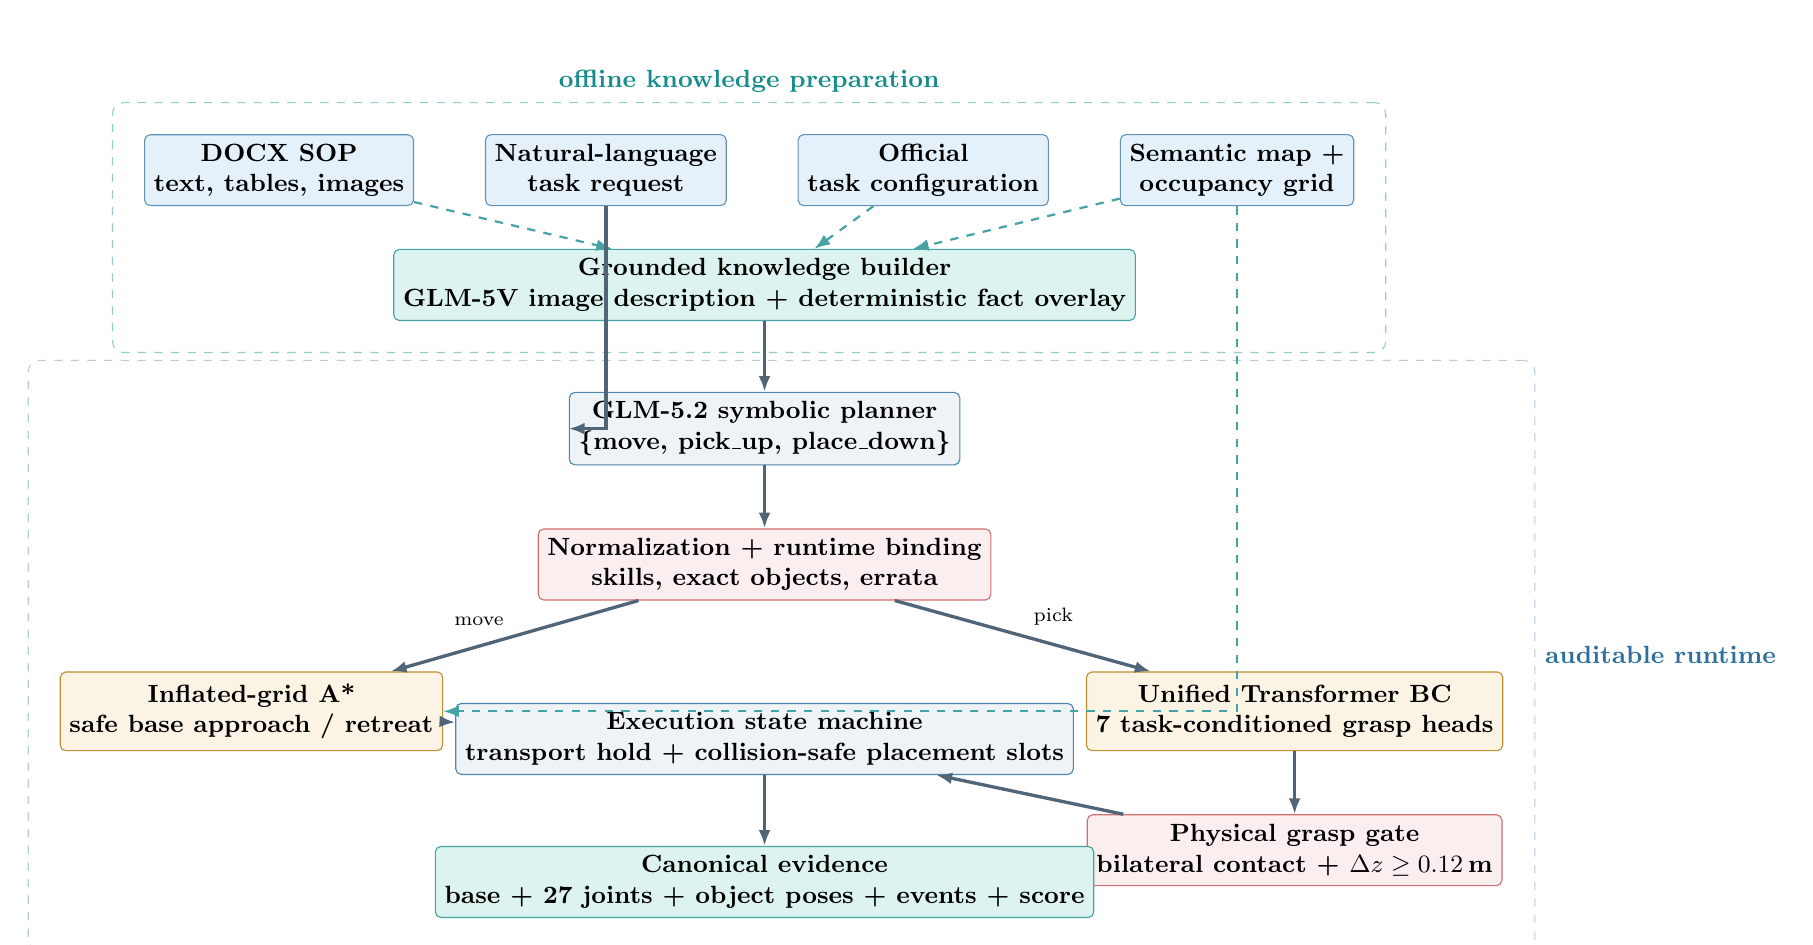
\begin{tikzpicture}[node distance=7mm and 9mm]
  \node[source] (sop) {DOCX SOP\\text, tables, images};
  \node[source,right=of sop] (prompt) {Natural-language\\task request};
  \node[source,right=of prompt] (cfg) {Official\\task configuration};
  \node[source,right=of cfg] (map) {Semantic map +\\occupancy grid};

  \node[offline,below=10mm of $(prompt)!0.5!(cfg)$] (ground) {Grounded knowledge builder\\GLM-5V image description + deterministic fact overlay};
  \node[runtime,below=9mm of ground] (planner) {GLM-5.2 symbolic planner\\\{move, pick\_up, place\_down\}};
  \node[verify,below=8mm of planner] (guard) {Normalization + runtime binding\\skills, exact objects, errata};
  \node[control,below left=9mm and 12mm of guard] (nav) {Inflated-grid A*\\safe base approach / retreat};
  \node[control,below right=9mm and 12mm of guard] (bc) {Unified Transformer BC\\7 task-conditioned grasp heads};
  \node[verify,below=8mm of bc] (physics) {Physical grasp gate\\bilateral contact + $\Delta z \geq 0.12$\,m};
  \node[runtime,below=13mm of guard] (exec) {Execution state machine\\transport hold + collision-safe placement slots};
  \node[offline,below=9mm of exec] (audit) {Canonical evidence\\base + 27 joints + object poses + events + score};

  \draw[dataflow] (sop) -- (ground);
  \draw[dataflow] (cfg) -- (ground);
  \draw[dataflow] (map) -- (ground);
  \draw[flow] (prompt) |- (planner);
  \draw[flow] (ground) -- (planner);
  \draw[flow] (planner) -- (guard);
  \draw[flow] (guard) -- node[above left,font=\scriptsize]{move} (nav);
  \draw[flow] (guard) -- node[above right,font=\scriptsize]{pick} (bc);
  \draw[flow] (nav) -- (exec);
  \draw[flow] (bc) -- (physics);
  \draw[flow] (physics) -- (exec);
  \draw[flow] (exec) -- (audit);
  \draw[dataflow] (map) |- (nav);

  \begin{scope}[on background layer]
    \node[fit=(sop)(map)(ground),draw=teal!45,dashed,rounded corners=4pt,inner sep=4mm,label={[font=\small\bfseries\color{teal}]above:offline knowledge preparation}] {};
    \node[fit=(planner)(guard)(nav)(bc)(physics)(exec)(audit),draw=blue!35,dashed,rounded corners=4pt,inner sep=4mm,label={[font=\small\bfseries\color{blue}]right:auditable runtime}] {};
  \end{scope}
\end{tikzpicture}}
\caption{System overview. Language models are restricted to knowledge extraction and symbolic planning; deterministic guards bind plans to official scene identities. Continuous grasping is delegated to BC, while physical measurements decide whether execution may transition to transport. Every cross-module decision is serialized into the trajectory evidence.}
\label{fig:overview}
\end{figure*}

\section{Problem Formulation}

For task $k$, the natural-language request defines an object set $\mathcal{O}_k$, source station $s_k$, and target station $g_k$. The agent emits a symbolic plan
\begin{equation}
\pi_k^{\text{sym}} = (a_1,\ldots,a_T), \qquad
a_t \in \{\textsc{Move},\textsc{Pick},\textsc{Place}\},
\end{equation}
then realizes each action through deterministic navigation or a learned continuous policy. A submitted trajectory contains frames
\begin{equation}
\tau_k = \{(t_i,\mathbf{b}_i,\mathbf{q}_i,\mathbf{X}_i, c_i)\}_{i=1}^{N_k},
\end{equation}
where $\mathbf{b}_i\in SE(3)$ is the base pose, $\mathbf{q}_i\in\mathbb{R}^{27}$ contains the recorded joints, $\mathbf{X}_i$ maps every movable object to an $xyz+xyzw$ pose, and $c_i$ is the collision flag. The objective score additionally depends on correctly named successful-grasp events, departure from the source, target proximity below 0.8\,m, and absence of collision flags.

The official scenes are fixed and expose semantic state. Our goal is therefore not open-world perception, but reliable transformation from SOP semantics to score-compatible physical execution.

\section{SOP Grounding and Planning}

\subsection{Two-stage evidence construction}

We separate contestant-authored offline grounding from the inherited online planner. The former parses paragraphs, tables, and de-duplicated figures from each official DOCX without reading the reference \code{sop*.md}. Zhipu \code{glm-5v-turbo} receives a narrow observation prompt---describe only visible layout, stations, objects, and legible labels---and is never used during trajectory replay. A text model then synthesizes concise Markdown from DOCX text, image observations, and read-only simulator/API facts. It must preserve quantity, use only the three executable skills, repeat a complete four-action cycle per distinct object, and distinguish document evidence from runtime metadata. Deterministic code prepends a \emph{Planner-Critical Facts} header containing level, exact source/target/object identities, quantity, model, and source hash; the model cannot overwrite this header. Outputs and provenance are retained in a manifest.

\subsection{Constrained GLM-5.2 planning}

The online template under \code{src/robot\_agent/core/} is unchanged from the official baseline. It forms one user message from bounded official knowledge (4,000 characters total, at most 600 per document), only the current row of \code{sop\_main.md}, a separate 4,000-character team-knowledge block, the live station-to-object map, registered skill schemas, one four-step JSON example, hard rules, and the current task. The general command, pick, place, and constraint documents are loaded for every level subject to this budget. Neither the entire task configuration nor a full semantic-map dump is inserted online; deterministic navigation consumes the map separately.

Reported executions use Zhipu \code{glm-5.2}~\citep{glm52docs} through an OpenAI-compatible protocol with temperature 0.1, 4,096 output tokens, JSON-object mode, and thinking disabled. ``OpenAI API'' in the UI denotes protocol compatibility, not an OpenAI model. Parsing attempts direct JSON, common syntax repairs, object extraction, and a bounded retry. The inherited normalizer validates registered skill names; execution fills missing object identities from the live map, applies narrow August-errata alias corrections, and preserves a distinct remaining-object order for L5. We do not claim universal pre-execution semantic verification of every field. Reliability instead comes from redundant prompt evidence, runtime binding, physical checks, and trajectory audit. Current retrieval is bounded rather than task-ranked and may include irrelevant cross-task snippets; this limitation and sanitized L3/L5 prompt examples are documented in \code{team\_submission/PROMPT\_DESIGN.md}. Once generated knowledge is present, the VLM is unnecessary for final execution.

\section{Navigation and Manipulation}

\subsection{Collision-aware base motion}

We parse each semantic station center and its occupancy grid, inflate obstacles by the robot footprint, and run A*~\citep{hart1968astar}. Execution separates global travel, a collision-free pre-approach, orientation matching to the BC deployment pose, and a safe retreat. Identity resolution performs exact matching before compatibility matching; this prevents names such as \code{aux\_output\_1} from being accidentally reduced to \code{output\_1}.

\subsection{Unified task-conditioned BC}

The continuous controller is implemented with robomimic~\citep{mandlekar2022robomimic} and PyTorch in robosuite/MuJoCo~\citep{zhu2020robosuite,todorov2012mujoco}. It follows the behavior-cloning paradigm~\citep{pomerleau1989alvinn} with a Transformer temporal backbone~\citep{vaswani2017attention}. At step $t$, the observation is
\begin{equation}
\mathbf{o}_t = [\mathbf{p}^{L,R}_{eef},\mathbf{r}^{L,R}_{eef},
\mathbf{q}^{L,R}_{grip},t,\mathbf{e}_k],
\end{equation}
where $\mathbf{e}_k\in\{0,1\}^7$ is the task identity. The policy predicts a 20-D bimanual action. It uses a four-layer, 256-D Transformer with eight attention heads and context length 10.

The deploy artifact is one checkpoint, not a bundle of seven independent networks. A 3,174,052-parameter shared encoder/Transformer feeds seven linear action heads totaling 35,980 parameters. Explicit output isolation was necessary because a single shared output layer produced destructive interference between geometrically similar observations requiring different approach actions. The resulting 3,210,032-parameter file occupies 12,928,025 bytes.

\begin{figure}[t]
\centering
\resizebox{\columnwidth}{!}{%
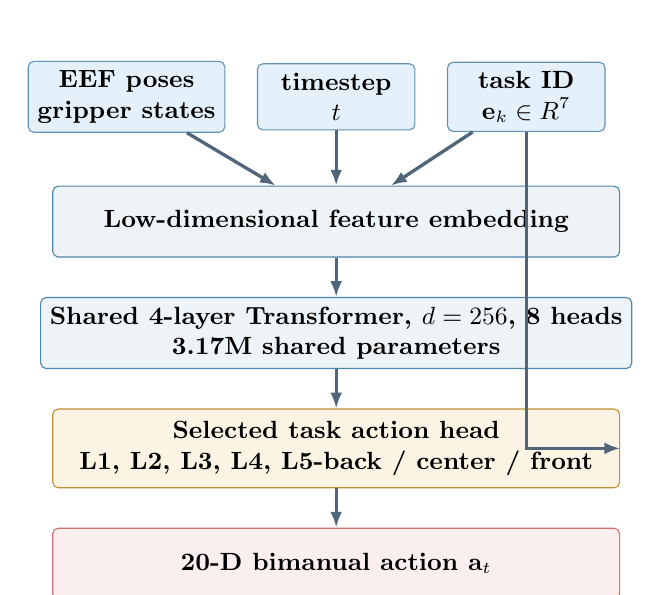
\begin{tikzpicture}[node distance=5mm]
  \node[source,minimum width=20mm] (state) {EEF poses\\gripper states};
  \node[source,minimum width=20mm,right=4mm of state] (time) {timestep\\$t$};
  \node[source,minimum width=20mm,right=4mm of time] (task) {task ID\\$\mathbf{e}_k\in\mathbb{R}^7$};
  \node[runtime,below=7mm of time,minimum width=72mm] (embed) {Low-dimensional feature embedding};
  \node[runtime,below=5mm of embed,minimum width=72mm] (trunk) {Shared 4-layer Transformer, $d=256$, 8 heads\\3.17M shared parameters};
  \node[control,below=5mm of trunk,minimum width=72mm] (heads) {Selected task action head\\L1, L2, L3, L4, L5-back / center / front};
  \node[verify,below=5mm of heads,minimum width=72mm] (action) {20-D bimanual action $\mathbf{a}_t$};
  \draw[flow] (state) -- (embed);
  \draw[flow] (time) -- (embed);
  \draw[flow] (task) -- (embed);
  \draw[flow] (embed) -- (trunk);
  \draw[flow] (trunk) -- (heads);
  \draw[flow] (task) |- (heads);
  \draw[flow] (heads) -- (action);
\end{tikzpicture}}
\caption{One deploy checkpoint shares temporal representation while isolating conflicting action mappings with seven lightweight heads. Task identity conditions both the input and head selection.}
\label{fig:bc}
\end{figure}

\subsection{Expert data and selection}

An analytic staged controller generates approach, alignment, finger closing, holding, and optional lifting actions. We perturb base $x/y$/yaw, phase duration, and action values. Episodes enter the corpus only when they pass bilateral pad contact, lift, and collision tests. The shared corpus contains 336 successful demonstrations and 174,860 steps (\cref{tab:data}). We additionally extract 144 real contact-closing windows (16,752 steps) to rebalance a physically critical phase that is short relative to the full trajectory.

\begin{table}[t]
\centering
\caption{Successful expert demonstrations used by the unified policy.}
\label{tab:data}
\small
\begin{tabular}{lrr}
\toprule
Branch & Episodes & Steps \\
\midrule
L1 & 48 & 15,015 \\
L2 & 48 & 22,789 \\
Corrected L3 & 48 & 23,819 \\
L4 & 48 & 24,277 \\
L5 back & 48 & 24,705 \\
L5 center & 48 & 32,596 \\
L5 front & 48 & 31,659 \\
\midrule
\textbf{Total} & \textbf{336} & \textbf{174,860} \\
\bottomrule
\end{tabular}
\end{table}

Training minimizes $\mathcal{L}=\mathcal{L}_2+0.1\mathcal{L}_1$. After joint training from random initialization, only the failing L2, corrected-L3, and L5-center heads are calibrated while the shared trunk and unrelated heads remain frozen. Selection is not based solely on validation loss: a checkpoint must pass the intersection of seven strict physical grasp-and-lift rollouts. For example, later L3 epochs achieved lower training progress yet lost bilateral contact; the earliest stable physically valid epoch was retained.

\subsection{Physics-gated transport}

The controller measures contact between both grippers' pad geometries and the target, then requires an approximately 0.12\,m object lift. Only after both tests pass does the existing competition transport attachment maintain the object during long-range base motion. Thus attachment stabilizes an already successful physical grasp; it does not replace grasping or recover a failed BC rollout. At the target, L5 objects are rotated and assigned non-overlapping offsets $[-0.55,0,+0.55]$\,m to prevent later placements from displacing earlier ones.

\section{Evaluation Protocol}

All final trajectories were generated after the official SOP correction. The canonical package contains the checkpoint hash, result JSON, full trajectory JSON, knowledge provenance, and rendered replay for each task. Our verifier independently checks:
\begin{itemize}
  \item checkpoint and evidence SHA-256 hashes;
  \item a base pose, the same 27 named joints, and all declared 7-D object poses in every frame;
  \item correctly named successful-grasp events and source departure;
  \item final target distance and collision flags; and
  \item the public scoring conditions for single- and multi-object tasks.
\end{itemize}
No LLM, VLM, MuJoCo process, or API key is required for this audit.

\begin{figure}[t]
\centering
\resizebox{\columnwidth}{!}{%
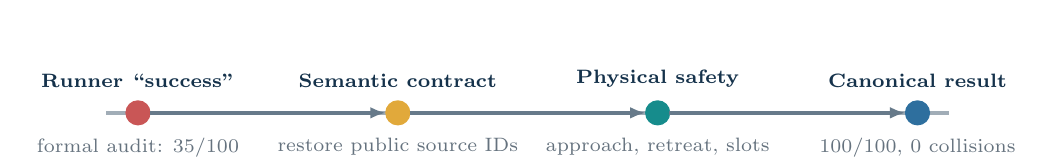
\begin{tikzpicture}
  \draw[very thick,navy!40] (0,0) -- (10.7,0);
  \foreach \x/\title/\detail/\tone in {
    0.4/{Runner ``success''}/{formal audit: 35/100}/rose,
    3.7/{Semantic contract}/{restore public source IDs}/gold,
    7.0/{Physical safety}/{approach, retreat, slots}/teal,
    10.3/{Canonical result}/{100/100, 0 collisions}/blue}
  {
    \fill[\tone] (\x,0) circle (0.16);
    \node[align=center,font=\scriptsize\bfseries,text=navy,above=2mm] at (\x,0) {\title};
    \node[align=center,font=\scriptsize,text=midgray,below=2mm] at (\x,0) {\detail};
  }
  \draw[->,very thick,navy!65] (0.55,0) -- (3.55,0);
  \draw[->,very thick,navy!65] (3.85,0) -- (6.85,0);
  \draw[->,very thick,navy!65] (7.15,0) -- (10.15,0);
\end{tikzpicture}}
\caption{Development audit. Execution completion and formal score were initially different notions. Explicit semantic and physical contracts turned scorer compatibility into a first-class regression test.}
\label{fig:timeline}
\end{figure}

\section{Results and Analysis}

\Cref{tab:results} reports the canonical evidence. Every task obtains its maximum score; all seven grasp branches pass BC contact-and-lift evaluation. L5 performs three complete cycles and is intentionally longer than the single-object tasks. Final L5 target distances are 0.583, 0.494, and 0.521\,m; the corrected L3 object ends 0.075\,m from its target center.

\begin{table*}[t]
\centering
\caption{Official-condition trajectory audit. ``BC + lift'' denotes bilateral physical contact and measured lift before transport hold.}
\label{tab:results}
\small
\begin{tabularx}{0.94\textwidth}{lrrrrXr}
\toprule
Task & Plan steps & Frames & Collision frames & Successful grasps & Manipulation mode & Score \\
\midrule
L1 & 4/4 & 304 & 0 & 1 & BC + physical lift & 10/10 \\
L2 & 4/4 & 344 & 0 & 1 & BC + physical lift & 15/15 \\
L3 & 4/4 & 360 & 0 & 1 & corrected blue tote, BC + physical lift & 20/20 \\
L4 & 4/4 & 367 & 0 & 1 & BC + physical lift & 25/25 \\
L5 & 12/12 & 974 & 0 & 3 & three BC grasps + separated placement slots & 30/30 \\
\midrule
\textbf{Total} & \textbf{28/28} & \textbf{2,349} & \textbf{0} & \textbf{7} & one unified checkpoint & \textbf{100/100} \\
\bottomrule
\end{tabularx}
\end{table*}

\begin{figure*}[t]
\centering
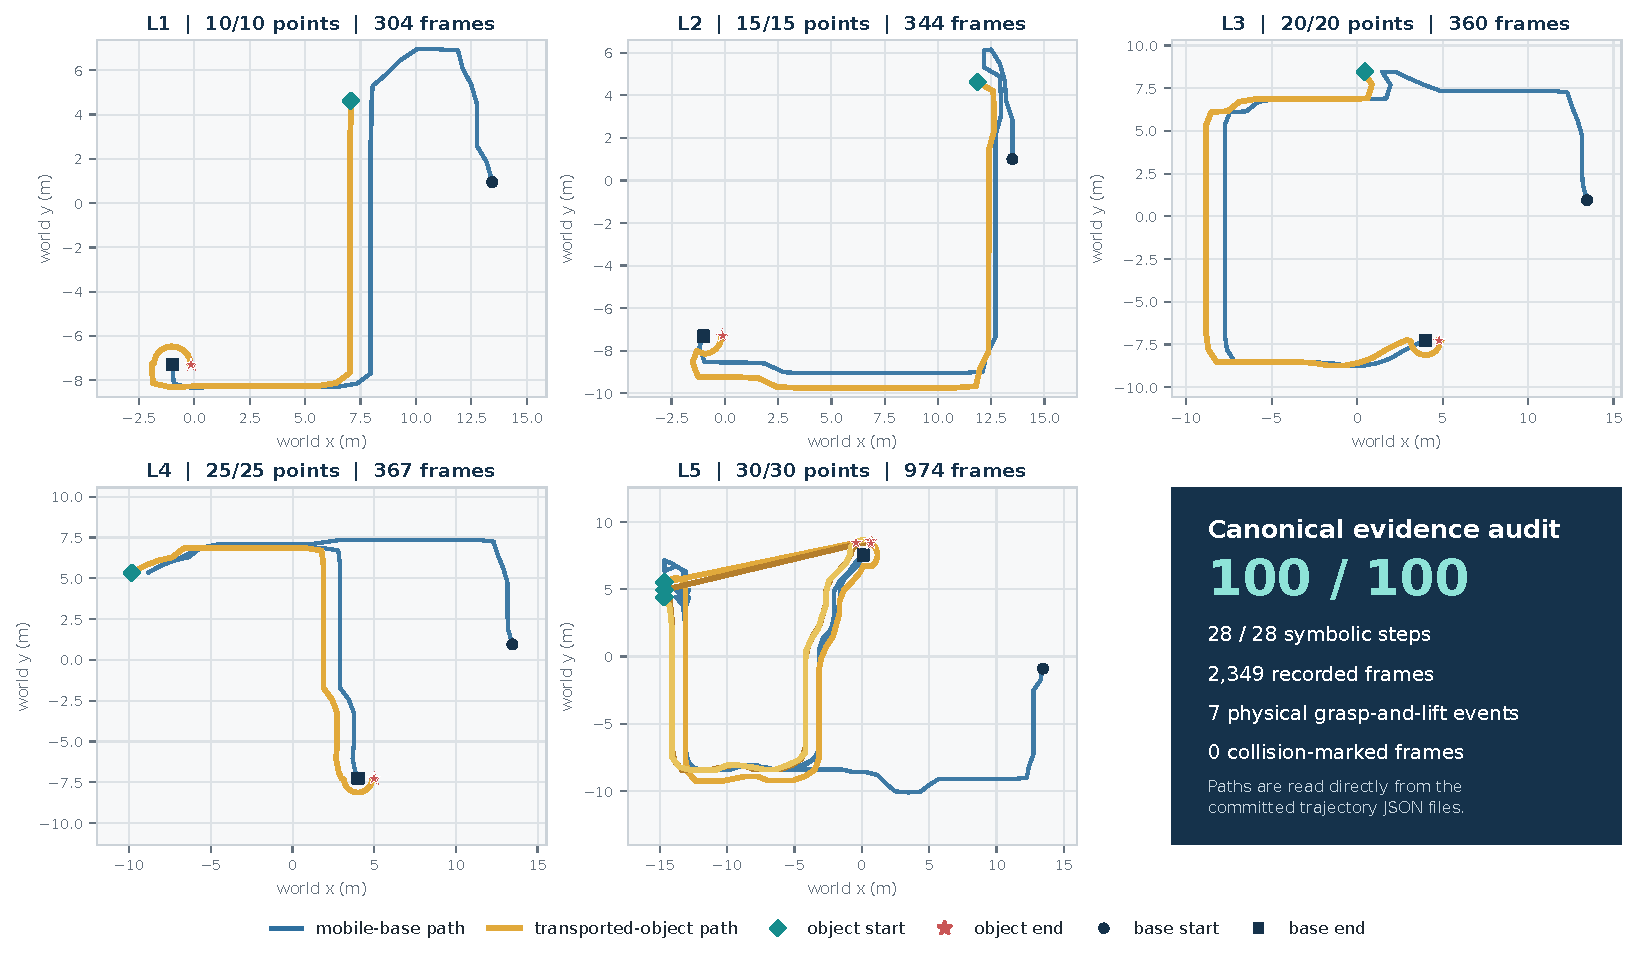
\includegraphics[width=0.84\textwidth]{figures/trajectory_gallery.pdf}
\caption{Canonical base and transported-object trajectories for all five tasks. The curves are generated directly from the committed trajectory JSON files; the dark panel summarizes the independently auditable outcome. L5 contains three distinct object paths because it performs three full transport cycles.}
\label{fig:trajectories}
\end{figure*}

\subsection{What mattered in optimization}

Three observations were more useful than adding model capacity. First, scorer-visible identities must be treated as a public interface: internal aliases may select a policy, but trajectory events must retain official station names. Second, only physically valid demonstrations should enter BC; low imitation loss does not imply bilateral contact. Third, multi-object placement is sequential interaction rather than three independent target checks. Explicit orientation and spatial slots eliminated object--object displacement.

The single-checkpoint design also clarifies the role of task conditioning. A one-hot identity alone did not fully prevent gradient conflict in the shared output map. Sharing temporal representation while isolating the final linear action maps preserved compact deployment and eliminated the observed cross-task output interference.

\subsection{Limitations}

The reported \score is one deterministic execution per fixed official scene, not a confidence interval across randomized environments. The low-dimensional policy uses simulator state and therefore cannot directly transfer to an RGB-only physical robot. Task-head selection assumes correct object identity. Long L5 replay is memory-intensive on CPU, and online planning latency depends on an external GLM service. Finally, physics-gated attachment is appropriate to the provided simulator but should not be confused with real-world force-controlled transport.

\section{Reproducibility and Compliance}

The public repository includes a 12.9\,MB checkpoint as an ordinary Git blob, five canonical trajectories, generated knowledge with provenance, GIF replays, all participant workflows, and a dependency-locked environment. Running
\begin{quote}\small\ttfamily
python team\_submission/verify\_submission.py
\end{quote}
recomputes the score without simulation or API access. GitHub Actions runs the same verifier on each push. The final checkpoint hash is
\begin{center}\scriptsize\ttfamily
f8c7feb8047ad62f4e1e01f0e67886a0\\
aa41f87781d486ae90e23164c37a7a5d
\end{center}
Expert HDF5 data are regenerated from fixed-seed simulator scripts; exact bytewise retraining is not promised across CUDA/MuJoCo platforms, while evaluation of the committed artifact is byte-exact.

{\raggedright The protected competition files---\code{app.py}, \code{src/robot\_agent/core}, \code{src/robot\_agent/environments}, and \code{knowledge/task\_config.json}---remain identical to the official functional base. Participant modifications are confined to skills, the isolated task runner, adjustable robot parameters, generated knowledge, and training/audit workflows.\par}

\section{Conclusion}

\method demonstrates that a fixed industrial manipulation benchmark benefits less from unconstrained end-to-end complexity than from explicit contracts between language, geometry, learned control, physics, and evaluation. Grounded GLM planning provides semantic flexibility; A* and a compact task-conditioned BC checkpoint provide executable motion; physical gates prevent silent grasp substitution; and trajectory auditing makes the final score reproducible. The resulting system reaches the maximum objective score while retaining an honest boundary around its fixed-scene evidence and transfer limitations.

\renewcommand{\bibfont}{\scriptsize}
\setlength{\bibsep}{1pt plus 0.3ex}
\bibliographystyle{abbrvnat}
\bibliography{references}

\end{document}
